\documentclass[11pt]{scrartcl} 


\usepackage{graphicx,graphics,tikz,pgfkeys}
\usetikzlibrary{arrows,decorations.pathreplacing}
\usepackage{amsmath}
\usepackage{amsthm}
\usepackage{amsfonts}
\usepackage{amssymb}
\usepackage{gensymb}



\usepackage{fixltx2e} % to be able to use the command \textsubscript

\usepackage[amssymb,thinqspace,textstyle,binary,noams,derivedinbase,derived]{SIunits} % To use SI units.
% amssymb: This option redefines the amssymb command \square to get
% the desired SIunits definition of the command.  Note: When using
% this option, the amssymb command \square can not be used.

%thinqspace This mode provides the use of \, (thin math space) as spacing be-
%        tween numerical quantities and units.

% textstyle:  When using the option textstyle units are printed in the typeface of the
%enclosing text, automatically.

%binary   This option loads the file binary.sty, which defines prefixes for binary
%         multiples.
%noams This option redefines the \micro command; use it when you don’t have
%         the AMS font, eurm10.
%derivedinbase This mode provides the ready-to-use expressions of SI derived units
%         in SI base units, e. g. \pascalbase to get ‘m−1 kg s−2 ’.
%derived This mode provides the ready-to-use expressions of SI derived units in SI
%         derived units, e. g. \derpascal to get ‘N m−2 ’.


%\usetikzlibrary{arrows,decorations.pathmorphing,backgrounds,placments,fit}
\usepackage[graphics,tightpage,active]{preview}
\PreviewEnvironment{tikzpicture}
\newlength\imagewidth
\newlength\imagescale

\begin{document}

sdssss\pgfmathsetlength{\imagewidth}{20cm} % desired displayed width of image
\pgfmathsetlength{\imagescale}{\imagewidth/1200} % pixel width of image
% adjust scale of tikzpicture (and direction of y) such that pixel
% coordinates can be used for drawing overlays:


\begin{center}
  \begin{tikzpicture}[font=\sffamily]

\begin{scope}
  \node[scale=1] at (0cm,1.7cm) {\textbf{Epigenetic distances}};
  \node[scale=1] at (0cm,1.2cm) {Genes (CG)};    

\begin{scope}
\node[inner sep=0pt,outer sep=0pt,scale=1] at (0cm,0cm) {
\includegraphics[width=1cm]{seagrass8.png}};
\draw [latex-latex,line width=0.02cm] (-0.3cm,-0.05cm) --  (-0.9cm,-0.35cm);
\node[inner sep=0pt,outer sep=0pt,scale=1] at (-1.2cm,-0.5cm) {
\includegraphics[width=1cm]{seagrass8.png}};
\draw [latex-latex,line width=0.02cm] (0.3cm,0.1cm) --  (0.9cm,0.4cm);
\node[inner sep=0pt,outer sep=0pt,scale=1] at (1.2cm,0.5cm) {
\includegraphics[width=1cm]{seagrass8.png}};
\end{scope}

\draw [-latex,line width=0.02cm] (-0.1cm,-0.8cm) -- node [scale=0.9,right=0.2cm]{Stress} (-0.1cm,-1.5cm);

\begin{scope}[yshift=-2cm]
\node[inner sep=0pt,outer sep=0pt,scale=1] at (0cm,0cm) {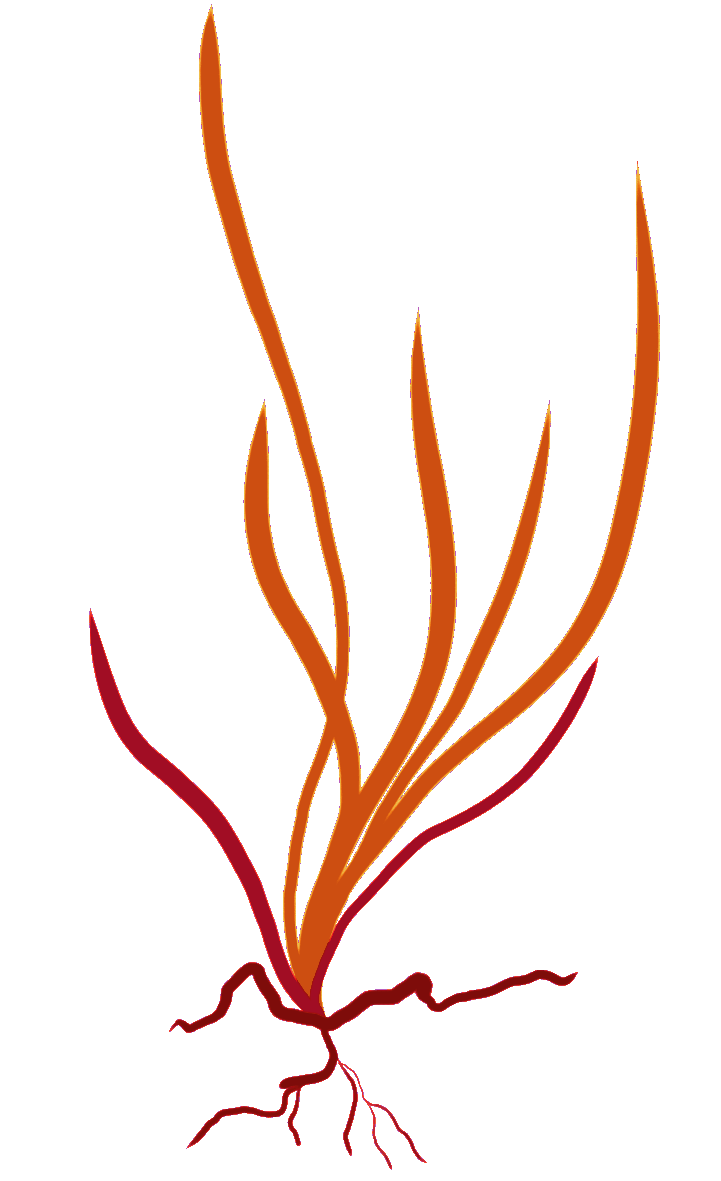
\includegraphics[width=1cm]{seagrass82.png}};
\draw [latex-latex,line width=0.02cm] (-0.3cm,-0.05cm) --  (-0.9cm,-0.35cm);
\node[inner sep=0pt,outer sep=0pt,scale=1] at (-1.2cm,-0.5cm) {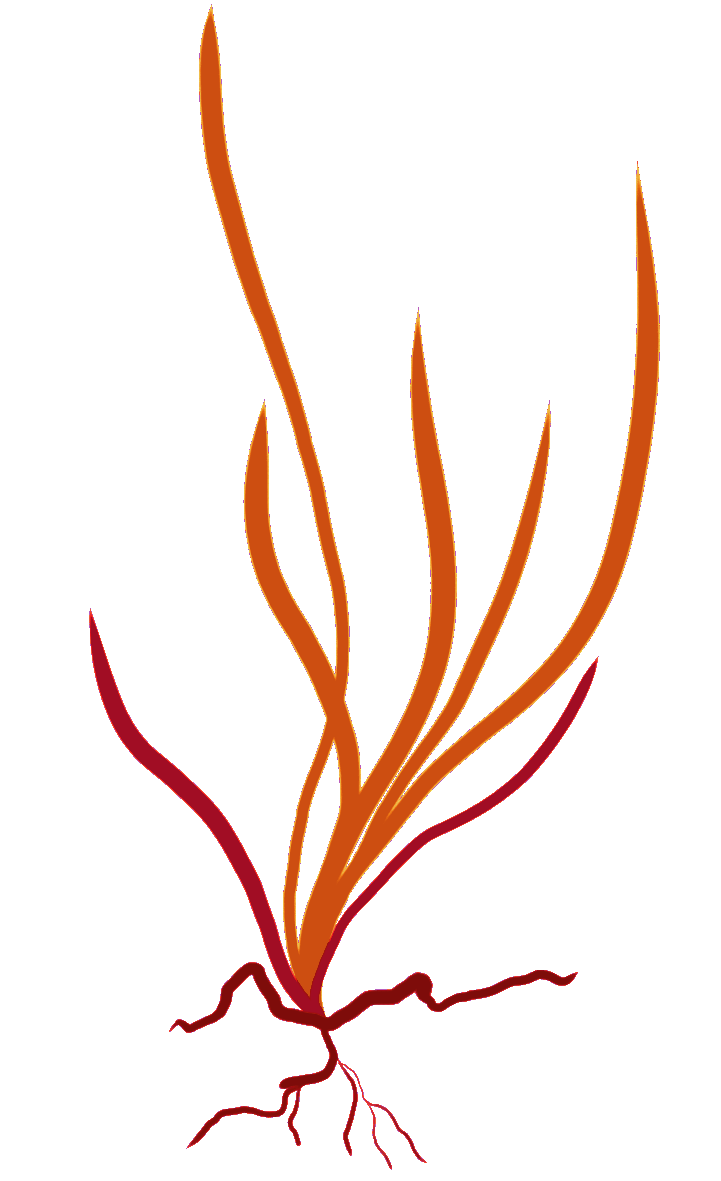
\includegraphics[width=1cm]{seagrass82.png}};
\draw [latex-latex,line width=0.02cm] (0.3cm,0.1cm) --  (0.9cm,0.4cm);
\node[inner sep=0pt,outer sep=0pt,scale=1] at (1.2cm,0.5cm) {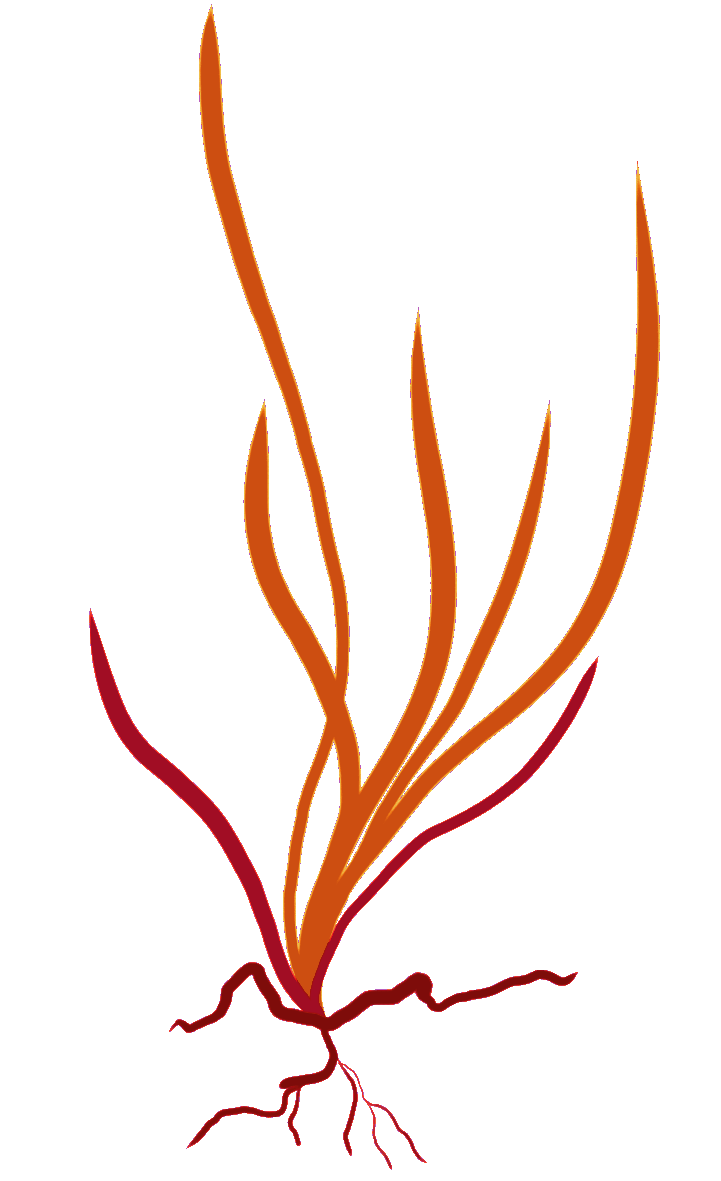
\includegraphics[width=1cm]{seagrass82.png}};
\end{scope}

\draw [-latex,line width=0.02cm] (-0.1cm,-2.8cm) -- node [scale=0.9,right=0.2cm]{Recovery} (-0.1cm,-3.5cm);

\begin{scope}[yshift=-4cm]
\node[inner sep=0pt,outer sep=0pt,scale=1] at (0cm,0cm) {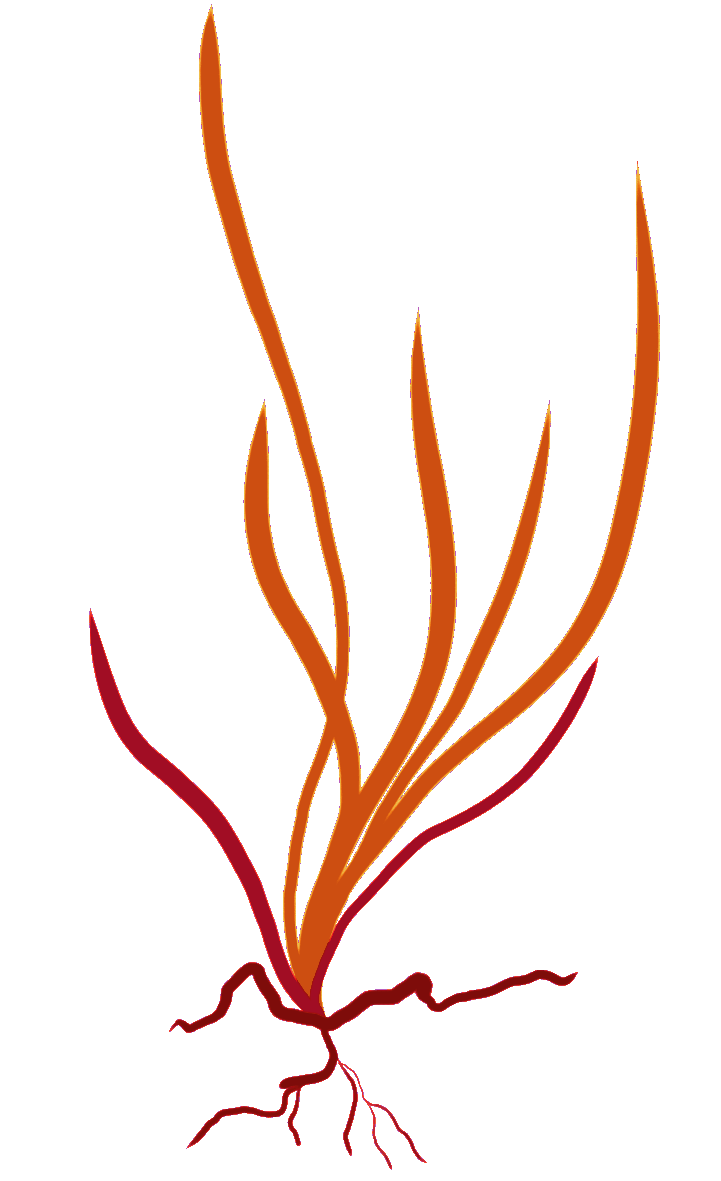
\includegraphics[width=1cm]{seagrass82.png}};
\draw [latex-latex,line width=0.02cm] (-0.3cm,-0.05cm) --  (-0.9cm,-0.35cm);
\node[inner sep=0pt,outer sep=0pt,scale=1] at (-1.2cm,-0.5cm) {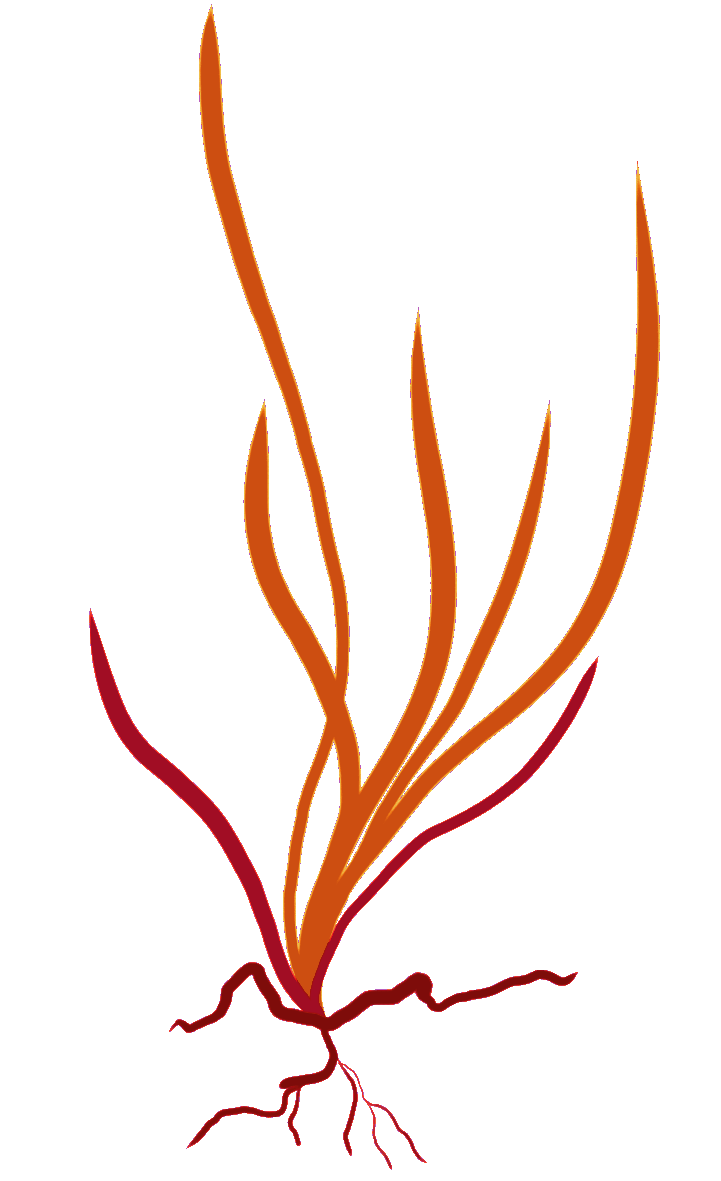
\includegraphics[width=1cm]{seagrass82.png}};
\draw [latex-latex,line width=0.02cm] (0.3cm,0.1cm) --  (0.9cm,0.4cm);
\node[inner sep=0pt,outer sep=0pt,scale=1] at (1.2cm,0.5cm) {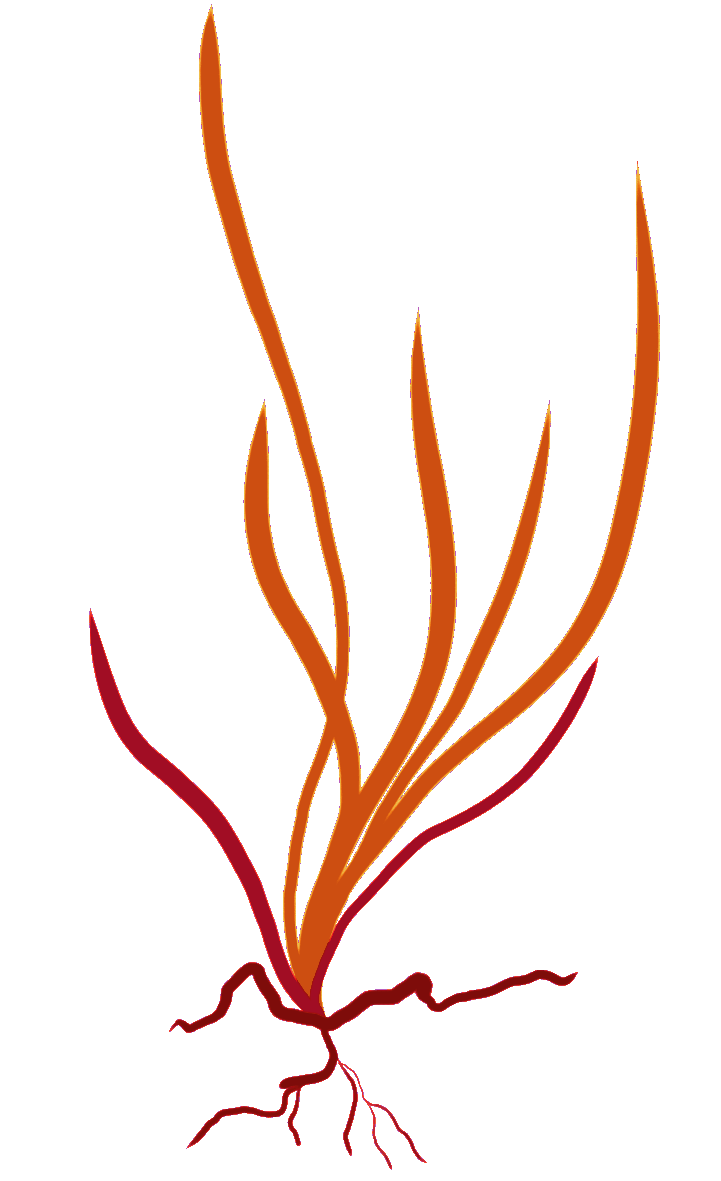
\includegraphics[width=1cm]{seagrass82.png}};
\end{scope}
\end{scope}


\draw [latex-latex,line width=0.02cm] (0.5cm,-0.2cm) -- node [scale=0.7,below=0.2cm]{correlated} (3.5cm,-0.5);

\draw [latex-latex,line width=0.02cm] (0.5cm,-0.2cm) -- node [scale=0.7,below=0.2cm,color=red!80!black]{correlated} (3.5cm,-4.5);


\begin{scope}[xshift=5cm]
\node[scale=1] at (0cm,1.7cm) {\textbf{Performance differences}};    

\begin{scope}
\node[inner sep=0pt,outer sep=0pt,scale=1] at (0cm,0cm) {
\includegraphics[width=1cm]{seagrass84.png}};
\draw [latex-latex,line width=0.02cm] (-0.3cm,-0.05cm) --  (-0.9cm,-0.35cm);
\node[inner sep=0pt,outer sep=0pt,scale=1] at (-1.2cm,-0.5cm) {
\includegraphics[width=1cm]{seagrass84.png}};
\draw [latex-latex,line width=0.02cm] (0.3cm,0.1cm) --  (0.9cm,0.4cm);
\node[inner sep=0pt,outer sep=0pt,scale=1] at (1.2cm,0.5cm) {
\includegraphics[width=1cm]{seagrass84.png}};
\end{scope}

\draw [-latex,line width=0.02cm] (-0.1cm,-0.8cm) -- node [scale=0.9,right=0.2cm]{Stress} (-0.1cm,-1.5cm);

\begin{scope}[yshift=-2cm]
\node[inner sep=0pt,outer sep=0pt,scale=1] at (0cm,0cm) {
\includegraphics[width=1cm]{seagrass83.png}};
\draw [latex-latex,line width=0.02cm] (-0.3cm,-0.05cm) --  (-0.9cm,-0.35cm);
\node[inner sep=0pt,outer sep=0pt,scale=1] at (-1.2cm,-0.5cm) {
\includegraphics[width=1cm]{seagrass83.png}};
\draw [latex-latex,line width=0.02cm] (0.3cm,0.1cm) --  (0.9cm,0.4cm);
\node[inner sep=0pt,outer sep=0pt,scale=1] at (1.2cm,0.5cm) {
\includegraphics[width=1cm]{seagrass83.png}};
\end{scope}

\draw [-latex,line width=0.02cm] (-0.1cm,-2.8cm) -- node [scale=0.9,right=0.2cm]{Recovery} (-0.1cm,-3.5cm);

\begin{scope}[yshift=-4cm]
\node[inner sep=0pt,outer sep=0pt,scale=1] at (0cm,0cm) {
\includegraphics[width=1cm]{seagrass84.png}};
\draw [latex-latex,line width=0.02cm] (-0.3cm,-0.05cm) --  (-0.9cm,-0.35cm);
\node[inner sep=0pt,outer sep=0pt,scale=1] at (-1.2cm,-0.5cm) {
\includegraphics[width=1cm]{seagrass84.png}};
\draw [latex-latex,line width=0.02cm] (0.3cm,0.1cm) --  (0.9cm,0.4cm);
\node[inner sep=0pt,outer sep=0pt,scale=1] at (1.2cm,0.5cm) {
\includegraphics[width=1cm]{seagrass84.png}};
\end{scope}
\end{scope}

\end{tikzpicture}


\end{center}

\end{document}